%%This is a very basic article template.
%%There is just one section and two subsections.
\documentclass{article}
\usepackage{graphicx}
\usepackage{amsmath}
\usepackage{mathtools}
\usepackage{color}
\begin{document}
\title{Photocurrent Action spectra of Photovotaic Devices}
\maketitle
\section{Internal Optical electric field and energy dissipation due to an incident plane wave
}
\subsection{Transfer Matrix Method:~\cite{pettersson1999modeling}}

Stratified structures can be described by $2\times2$ matrix 
due to the fact that the equation governing the propagation 
of the electric field are linear and that the tangential component 
of the electric field is continuous.Consider a plane wave incident from left at a general multilayer 
structure having m layers between a semi-infinite transparent ambient 
and a semi-infinite substrate as schematically described in Figure
\ref{fig:layers}.
\begin{figure}[h!]
  \centering
    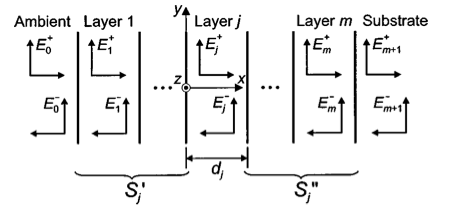
\includegraphics[width=0.7\textwidth]{layers}
  \caption{A general multilayer structure having m layers between a semi 
  infinite transparent ambient and a semi-infinite substrate. 
 Each layer j(j=1,2,…,m) has a thickness $d_{j}$ and its optical properties are
 described by its complex index of refraction. The optical electric field at any
 point in lyaer j is represented by two components: one propagating in the
 positive and one in the negative x direction, $\mathbf{E_{j}^{+}}$ and
 $\mathbf{E_{j}^{-}}$, respectively} \label{fig:layers} 
\end{figure}
\subsubsection{Theoretical Background}
\textbf{Internal Optical Electric Field:}

The electric field in layer j can be expressed in terms of the matrix elements
of the partial system transfer matrices as

\begin{equation}
{{E}_{j}}(x)=\frac{S_{j11}^{''}\cdot {{e}^{-i{{\xi
}_{j}}({{d}_{j}}-x)}}+S_{j21}^{''}\cdot {{e}^{i{{\xi }_{j}}({{d}_{j}}-x)}}}{S_{j11}^{'}S_{j11}^{''}\cdot {{e}^{-i{{\xi }_{j}}{{d}_{j}}}}+S_{j12}^{'}S_{j21}^{''}\cdot {{e}^{i{{\xi }_{j}}{{d}_{j}}}}}E_{0}^{+}
\label{mainequation} 
\end{equation}
In Equation \ref{mainequation}:

$d_j$ is the thickness of the jth layer as shown in Figure \ref{fig:layers}.
\begin{equation}
{{\xi }_{j}}=\frac{2\pi }{\lambda }{{q}_{j}}
\end{equation}
\begin{equation}
S_{j}^{'}=\left[ \begin{matrix}
   S_{j11}^{'} & S_{j12}^{'}\\
   S_{j21}^{'} & S_{j22}^{'}  
\end{matrix} \right]=\left( \prod\limits_{v=1}^{j-1}{{{I}_{(v-1)v}}{{L}_{v}}} \right)\cdot {{I}_{(j-1)j}}
\label{Sp} 
\end{equation}
\begin{equation}
S_{j}^{''}=\left[ \begin{matrix}
   S_{j11}^{''} & S_{j12}^{''}\\
   S_{j21}^{''} & S_{j22}^{''}\\
\end{matrix} \right]=\left( \prod\limits_{v=j+1}^{m}{{{I}_{(v-1)v}}{{L}_{v}}} \right)\cdot {{I}_{m(m+1)}}
\label{Spp} 
\end{equation}
\begin{equation}
{{I}_{jk}}=\frac{1}{{{t}_{jk}}}\left[ \begin{matrix}
   1 & {{r}_{jk}}  \\
   {{r}_{jk}} & 1  \\
\end{matrix} \right]
\end{equation}
\begin{equation}
{{L}_{j}}=\left[ \begin{matrix}
   {{e}^{-i{{\xi }_{j}}{{d}_{j}}}} & 0  \\
   0 & {{e}^{i{{\xi }_{j}}{{d}_{j}}}}  \\
\end{matrix} \right]
\end{equation}
For light with the electric field perpendicular to the plane of
incidence(s-polarized or TE waves), the Fresnel complex reflection and
transmission coefficients are defined by
\begin{subequations}
\begin{equation}
{{r}_{jk}}=\frac{{{q}_{j}}-{{q}_{k}}}{{{q}_{j}}+{{q}_{k}}}
\end{equation}
\begin{equation}
{{t}_{jk}}=\frac{2{{q}_{j}}}{{{q}_{j}}+{{q}_{k}}}
\end{equation}
\end{subequations}
and for light with the electric field parallel to the plane of
incidence(p-polarized or TM waves) as
\begin{subequations}
\begin{equation}
{{r}_{jk}}=\frac{\tilde{n}_{k}^{2}{{q}_{j}}-\tilde{n}_{j}^{2}{{q}_{k}}}{\tilde{n}_{k}^{2}{{q}_{j}}+\tilde{n}_{j}^{2}{{q}_{k}}}
\end{equation}
\begin{equation}
{{t}_{jk}}=\frac{2{{{\tilde{n}}}_{j}}{{{\tilde{n}}}_{k}}{{q}_{j}}}{\tilde{n}_{k}^{2}{{q}_{j}}+\tilde{n}_{j}^{2}{{q}_{k}}}
\end{equation}
\end{subequations}
where
\begin{equation}
{{q}_{j}}={{\tilde{n}}_{j}}\cos {{\phi }_{j}}={{[\tilde{n}_{j}^{2}-\eta
_{0}^{2}\sin {{\phi }_{0}}]}^{1/2}}
\end{equation}
\textbf{Energy dissipation:}

Since the number of excitred state at a given position in a structure is
directly dependent on the energy absorbed by the material, the energy
dissipation of the electromagnetic field in the material is the quantity that is
of interest in the case of photovoltaic devices. The time average of the energy
dissipated per second in layer j at position x at normal incidence is given
by(c, speed of light; ${{\varepsilon }_{0}}$, permittivity of free space)
\begin{equation}
{{Q}_{j}}(x)=\frac{1}{2}c{{\varepsilon }_{0}}{{\alpha }_{j}}{{\eta
}_{j}}{{\left| {{E}_{j}}(x) \right|}^{2}}
\end{equation}
This means that the energy absorbed at position xin the layered structure is
proportional to the product of the modulus squared of the electric field
${{\left| {{E}_{j}}(x) \right|}^{2}}$, the refractive index ${{\eta }_{j}}$ and
the absorption coefficient
\begin{equation}
{{\alpha }_{j}}=\frac{4\pi {{\kappa }_{j}}}{\lambda }
\end{equation}
at the actual positon x.


\subsubsection{IOEF(Internal Optical Electric Field) Class Reference}
This class is written in Python 2.7.6, you can use this class to obtain internal
optical electric field due to an oncident plane wave
within the structure you defined in the class attributes.

\textbf{Instance Attributes:(id, phi0, wavelength, TME)}

\textcolor{blue}{id:} Define the Structure with a numpy.array Type.

\textcolor{blue}{phi0:} Define the incidence angle.

\textcolor{blue}{wavelength:} Define the wavelength.

\textcolor{blue}{TME:} Define the plorization of light (TE or TM).

\textbf{Method:}

\textcolor{blue}{EFfunc(j,x):} Get the electric field distributon at x in layer
j

\textcolor{blue}{plotEFfunc(layer):}Plot the electric field distribution vs x in
layer j
\subsubsection{Photocurrent Class Reference}
This class is a subclass of IOEF class, you can use this class to obtain the
enrgy dissipation of the electromagnetic field in the material and the
generated photocurrent at the active layer interface.

\textbf{Instance Attributes:(id, phi0, wavelength, TME)}

\textcolor{blue}{id:} Define the Structure with a numpy.array Type.

\textcolor{blue}{phi0:} Define the incidence angle.

\textcolor{blue}{wavelength:} Define the wavelength.

\textcolor{blue}{TME:} Define the plorization of light (TE or TM).

\textbf{Attributes:}

\textcolor{blue}{$\theta1$:} The quantum efficiency of the exction
generation(default value:1.0).

\textcolor{blue}{$\theta2$:} The efficiency of the exction dissociation at the
interface(default value:1.0).

\textcolor{blue}{D:} The diffusion constant(default
value:$18*10^{-8}$)

\textcolor{blue}{t:} The mean lifetime of the excition(default
value:$18*10^{-10}$s).

\textcolor{blue}{N:} Incident photon flux (default value:$2.365\times
{{10}^{18}}(W/{{m}^{2}}\cdot s)$).

\textcolor{blue}{dthickness:} Thickness of the activelayer(setting required).

\textcolor{blue}{layer:} Which layer is the activelayer(setting required).

\textbf{Method:}

\textcolor{blue}{Qjfunc:} get the Energy dissipation of the electromagnetic
field.

\textcolor{blue}{JPhotonfunc0:} get the generated short-circuit photocurrent
density at x=0.

\textcolor{blue}{JPhotonfuncd:} get the generated short-circuit photocurrent
density at x=dthickness.

\textcolor{blue}{JPhotonfuncd:} get the generated short-circuit photocurrent
density at x=dthickness.

\textcolor{blue}{ipce0:} get the incident monochromatic photon to current
collection efficiency(no reflection) at x=0

\textcolor{blue}{ipced:} get the incident monochromatic photon to current
collection efficiency(no reflection) at x=dthickness.

\subsubsection{Simulation Example}
\begin{figure}[h!]
  \centering
    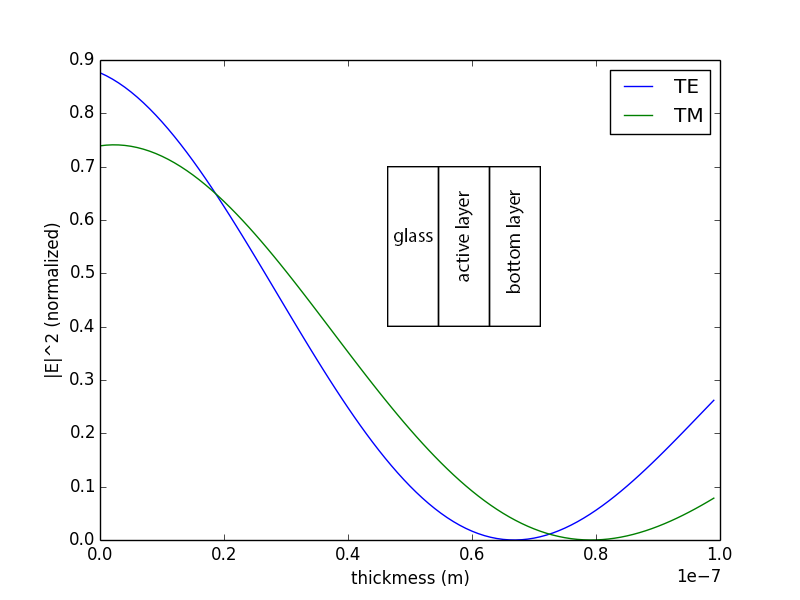
\includegraphics[width=1\textwidth]{electricfield}
  \caption{Calculated distribution of the normalized modulus squared of the
  optical electric field ${{\left| E \right|}^{2}}$(both TE and
  TM,$\lambda$=500nm) inside active layer as shown in the
  device(glass(semi-inifi,n=1.45)/active layer(t=100nm,n=1.8+0.2i)/bottom
  layer(t=500nm,n=1.2)/air), which is schenatically presented in the right
  corner.
  }
  \label{electricfield}
\end{figure}





\section{Exciton transport-diffusion equation
}
\subsection{Diffusion Equation Method~\cite{pettersson1999modeling}}
\subsubsection{Theoretical Background}
Consider photogenerated excitons formed by photoexcitation within an active
layer. The excitons can diffuse from the position where they were created and
be dissociated by interaction of the exciton at interfaces, impurities or
defects. After the dissociation of the exciton, charge collection is possible.
If n is the exciton density the diffusion equation gives
\begin{equation}
\frac{\partial n}{\partial t}=D\frac{{{\partial }^{2}}n}{\partial
{{x}^{2}}}-\frac{n}{\tau }+\frac{{{\theta }_{1}}}{hv}Q(x)
\label{diffusionequation} 
\end{equation}
where D is the diffusion constant,$\tau$ is the mean lifetime of the exciton,
$\theta_1$ is the quantum efficiency of the exciton generation, and $hv$ is the
excitation energy of the incident light. In Equation \ref{diffusionequation} the
first term on the right represents excitons moving away by diffusion, the second
term is a recombination term, and the third term represents the generation rate
of excitons(photogeneration). At steady state (equilibrium), the exciton density
is time independent and Equation \ref{diffusionequation} can be written as
\begin{equation}
\frac{{{d}^{2}}n}{d{{x}^{2}}}={{\beta }^{2}}n(x)-\frac{{{\theta
}_{1}}}{Dhv}Q(x)
\label{timeindependentdiffusionequation} 
\end{equation}
where $\beta =1/L=1/\sqrt{D\tau }$, i.e., the reciprocal of the diffusion length
L. The general solution to Equation \ref{timeindependentdiffusionequation} with
the generation terms given by the normal incidence case is
\begin{equation}
\begin{multlined}
   {{Q}_{j}}(x)={{\alpha }_{j}}{{T}_{j}}{{I}_{0}}[{{e}^{-{{\alpha }_{j}}x}}+\rho _{j}^{''2}\cdot {{e}^{-{{\alpha }_{j}}(2{{d}_{j}}-x)}}+2\rho _{j}^{''}\cdot {{e}^{-{{\alpha }_{j}}{{d}_{j}}}} \\ 
  \cdot \cos \left( \frac{4\pi \eta }{\lambda }({{d}_{j}}-x)+\delta _{j}^{''} \right)]  
\end{multlined}
\end{equation}

\begin{equation}
\begin{multlined}
   n(x)=\frac{{{\theta }_{1}}\alpha TN}{D({{\beta }^{2}}-{{\alpha }^{2}})}[A\cdot {{e}^{-\beta x}}+B\cdot {{e}^{\beta x}}+{{e}^{-\alpha x}}+{{C}_{1}}{{e}^{\alpha x}} \\ 
  +{{C}_{2}}\cdot \cos \left( \frac{4\pi \eta }{\lambda }({{d}_{j}}-x)+\delta _{j}^{''} \right)] \\ 
\end{multlined}
\label{exctiondensity}
\end{equation}
where N is the number of incident photons at the device per unit time per unit
area (incident photon flux).$I_0$ is the intensity of the incident
light,${{T}_{j}}=\left( {{\eta }_{j}}/{{\eta }_{0}} \right){{\left| t_{j}^{+}
\right|}^{2}}$ is the internal intensity transmittance, and $\rho _{j}^{''}$ and
$\delta _{j}^{''}$ are the absolute value and theargument of the complex
reflection coefficnent given by Equation \ref{rpp} , A and B are constants given
by the boundary condition in the model and
\begin{equation}
r_{j}^{'}=\frac{S_{j21}^{'}}{S_{j11}^{'}}
\end{equation}
\begin{equation}
t_{j}^{'}=\frac{1}{S_{j11}^{'}}
\end{equation}
\begin{equation}
r_{j}^{''}=\frac{S_{j21}^{''}}{S_{j11}^{''}}
\label{rpp}
\end{equation}
\begin{equation}
t_{j}^{''}=\frac{1}{S_{j11}^{''}}
\end{equation}
\begin{equation}
t_{j}^{''}=\frac{1}{S_{j11}^{''}}
\end{equation}
\begin{equation}
r_{{{j}^{-}}}^{'}=-S_{j12}^{'}/S_{j11}^{'}
\end{equation}
\begin{equation}
t_{j}^{+}=\frac{t_{j}^{'}}{1-r_{{{j}^{-}}}^{'}r_{j}^{''}\cdot {{e}^{i2{{\xi
}_{j}}{{d}_{j}}}}}
\end{equation}
\begin{equation}
{{C}_{1}}={{\rho }^{''2}}{{e}^{-2\alpha d}}
\end{equation}
\begin{equation}
{{C}_{2}}=\frac{({{\beta }^{2}}-{{\alpha }^{2}})}{({{\beta }^{2}}+{{(4\pi \eta /\lambda )}^{2}})}2{{\rho }^{''}}{{e}^{-\alpha d}}
\end{equation}
Assuming that the interface of the activelayer act as perfect sinks for the
excitons, i.e., all excitons can either recombine or dissociate into free
charges at the interfaces resulting in boundary condition n=0 at x=0 and x=d.
Solving for the two constant A and B using these boundary conditions together
with Equation \ref{exctiondensity}, the result becomes
\begin{equation}
A=\frac{({{e}^{\beta d}}-{{e}^{-\alpha d}})+{{C}_{1}}({{e}^{\beta
d}}-{{e}^{\alpha d}})+{{C}_{2}}\left[ {{e}^{\beta d}}\cdot \cos \left( \frac{4\pi \eta }{\lambda }d+{{\delta }^{''}} \right)-\cos ({{\delta }^{''}}) \right]}{({{e}^{-\beta d}}-{{e}^{\beta d}})}
\end{equation}
and
\begin{equation}
B=-\frac{({{e}^{-\beta d}}-{{e}^{-\alpha d}})+{{C}_{1}}({{e}^{-\beta
d}}-{{e}^{\alpha d}})+{{C}_{2}}\left[ {{e}^{-\beta d}}\cdot \cos \left( \frac{4\pi \eta }{\lambda }d+{{\delta }^{''}} \right)-\cos ({{\delta }^{''}}) \right]}{({{e}^{-\beta d}}-{{e}^{\beta d}})}
\end{equation}
The short-circuit exctiton current density at the interface x=0 can be found as
\begin{equation}
{{J}_{Exc}}={{\left. D\frac{dn}{dx} \right|}_{x=0}}
\end{equation}
which is related to the short-circuit photocurrent through
${{J}_{Photon}}=q{{\theta }_{2}}{{J}_{Exc}}$, where q is the electron charge and
$\theta_2$ is the efficiency of the exciton dissociation at the interface. The
resulting short-circuit photocurrent density generated at this interface
therefore is 
\begin{equation}
{{\left. {{J}_{Photon}} \right|}_{x=0}}=\frac{q\theta \alpha TN}{({{\beta
}^{2}}-{{\alpha }^{2}})}\left( -\beta A+\beta B-\alpha +\alpha {{C}_{1}}+\frac{4\pi \eta }{\lambda }{{C}_{2}}\cdot \sin \left[ \frac{4\pi \eta }{\lambda }d+{{\delta }^{''}} \right] \right)
\end{equation}
\bibliography{mybib}{}
\bibliographystyle{plain}
\end{document}
